%!TEX root = ThesisEx.tex

% \resetdatestamp

% Don't know what these three lines are, they came with the McGill template
% \newcommand\Dfrac[2]{\frac{\displaystyle #1}{\displaystyle #2}}
% \newcommand{\mathBF}[1]{\mbox{\boldmath $#1$}}
% \newcommand{\C}[1]{\mathBF{#1}}

\chapter{Music listening histories dataset}\label{ch:5-music-listening-histories-dataset}
\graphicspath{{./figs/ch7/} }
Music listening profiles are sources of behavioural information that can be used for understanding when and where people listen to music. 
% In addition, knowing when and where people listen to music are important contextual dimensions that can be used to improve the performance of context-aware music recommendation systems.
We are interested in evaluating the impact of using demographic and profiling features, as well as contextual information, for a large number of people, on the prediction accuracy of a music artist recommendation model. A few publicly available datasets for music listening research provide information relating people and music items. \textcite{dror11yahoo} presented a dataset of 1M people's aggregated ratings on music items. \textcite{mcfee12million} introduced a dataset of song playcounts of 1M listeners. Neither of these two datasets, however, provided timestamps of the music logs or demographic information about the listeners. \textcite{celma10music} provided a dataset of playcounts with listeners' demographic data for 360K listeners and a set of listening histories with full time-stamped logs; however this dataset only included logs for 1K listeners. \textcite{cantador11workshop} presented another small dataset with song playcounts for 2K listeners.
Finally, the Electric and Musical Industries (EMI) group promised a dataset of 1M interviews about people's music appreciation, behaviour, and attitudes \autocite{emi12million}, but only partial information was made available.

None of the aforementioned datasets simultaneously provided full music listening histories as well as demographic data for a large amount of listeners. 
This means it is not possible to extract all of the user-centric features that we are interested in, and so we decided to collect our own dataset made with music listening histories from the Last.fm music service.



% All data collected for the research project can be freely accessed thought the Last.fm API. At registration moment, every user must accept the Last.fm Terms of Use\footnote{Available at \url{http://www.last.fm/legal/terms#para7}} and the Last.fm Privacy Policy\footnote{Available at \url{http://www.last.fm/legal/privacy}}. Among other things, these terms establish that the listening habit data of listeners will be available to other Last.fm users and to third parties via their application programming interface (API) for commercial and/or non-commercial purposes.
% As a result, the information we will gather is contemplated on Article 2.2 of the \textcite{TCPS14ethics} and ``is considered to be publicly available information and therefore does not need ethics review.''\footnote{This is the response we received from the McGill University Research Ethics Board Associate Director via email.}





In this chapter we will describe the creation of a large dataset (N=594K) of full music listening histories. Section \ref{sec:5-dataset-collection} presents the criteria for the collection, the data acquisition, the cleaning, and the integration of the data. Section \ref{sec:5-dataset-demographics} provides insights about the demographic characteristics of users in the dataset. Section \ref{sec:5-temporal-alignment-of-music-listening-histories} presents the different approaches we investigated for performing a temporal alignment of the music listening histories in order to compare them directly.



% implemented six approaches for the identification of the time zones they were generated.
% The performance of these approaches was calculated in a dataset of listening profiles with manually labelled time zones. 
% Based on the assumption that people across the world share a relative moment during the night when they sleep and submit fewer music logs, the best method resulted in a 75 percent of correctly recognized time zones with a tolerance of $\pm$1 hour.






\section{Dataset collection}\label{sec:5-dataset-collection}  % From vigliensoni14always.tex
Last.fm is an online digital music service that has been available since October 2002. The company has been working uninterruptedly since then and has more 70 million registered users from 240 different countries.\footnote{Data retrieved using the Last.fm API on April 21, 2014} 
It was originally conceived as a web-based radio station that provided listeners with the possibility to skip songs or 'love' them. Immediately after their launch, Last.fm started integrating listening data from Audioscrobbler, a small company that tracked music listening logs by means of a background process application that runs in various media players. The two companies eventually merged and Last.fm incorporated the tracking of  music listening logs as a core part of their service.

Last.fm stands out from most online digital music services because it not only gathers listening logs from the interaction of Last.fm users and the Last.fm online music service, 
but also from the interaction between people and a wide range of music and media players by means of the \emph{scrobbler} application programming interface (API) service. 
The scrobbler service automatically submits a log to the listener's profile in the Last.fm database for each track played back in the user's listening device, what was defined by Last.fm as ``to scrobble.'' 
Since this service can be accessed by means of an API, third-party media players and online services do not necessarily need to install any software application in order to track listening logs.
As a result, the scrobbler service has been incorporated in more than than 600 digital music services, browsers, media players, and devices, such as Google Android, iOS,  Firefox, Google Chrome, Spotify, Pandora, Rdio, iTunes, Amazon Cloud, Squeezebox, and many others.\footnote{Partial list of scrobblers available at \url{http://build.last.fm/category/Scrobblers}} 

Last.fm offers free access to the listening data they collect as well as other information such as music metadata, biographies, pictures, charts, tags, as well as ranking data by country, by means of a well-documented API.\footnote{Last.fm API and Web services available at \url{http://www.last.fm/api}} 
% The data we want to collect for this research project can be freely accessed thought the Last.fm API. 
At the moment of registration, every user must accept the Last.fm Terms of Use\footnote{Last.fm Terms of Use available at \url{http://www.last.fm/legal/terms}} and the Last.fm Privacy Policy.\footnote{Last.fm Privacy Policy available at \url{http://www.last.fm/legal/privacy}} Among other things, these terms establish that the listening habit data of listeners will be available to other Last.fm users and to third parties via their API for commercial and/or non-commercial purposes.
As a result, the information we will gather is contemplated on Article 2.2 of the Canadian Tri-council policy statement on Ethical conduct for research involving humans \autocite{TCPS14ethics} 
and ``is considered to be publicly available information and therefore does not need ethics review.''\footnote{Response received via email from the McGill University Research Ethics Board Associate Director.}
% The Last.fm API Terms of Service establish that Last.fm offers to the users a ``limited terminable licence to copy and use the Last.fm Data'', which is free of charge but ``solely for non-commercial purposes.''~\footnote{\url{http://www.last.fm/api/tos}}
Since in the context of this research we do not plan to create a commercial product, and Last.fm gives us access to a large amount of interactions between listeners and wide array of digital music services, we decided to use the data they have collected for years.

Now, we will describe the criteria and acquisition methods that we used to collect the music listening histories for our dataset.







\subsection{Data criteria and acquisition}
Listening histories are a timeline of listening events that may reflect  aspects of when people consume music, and what music they enjoy or do not enjoy. Analysing them in a linear fashion is interesting because we can observe them as a series of listening events over time. 
However, the aggregation of these listening histories by collapsing them into periods of time can provide extra layers of information. As people usually follow periodic cycles, the analysis of these listening cycles can be used to infer their listening patterns. 

In order to obtain even data across aggregated periods of time---but also to reduce bias due to the novelty effect and allow for long-term conclusions---we followed the approach by \textcite{baur12listening} and searched only for listeners with a minimum of two years of activity since they scrobbled for the first time.
% with at least two years of activity submitting music logs since their first scrobble was submitted. 
Also, we only searched for listeners with an arbitrary minimum of 10 scrobbles per day in order to ensure they have been actively submitting music logs. 
With these restrictions we got rid of having listeners in our dataset   that registered for a service, tried it, and never used it again.  The two constraints forced all listeners in our dataset to have a minimum of 7,300 (i.e., 365 $\times$ 2 $\times$ 10) music logs submitted to the Last.fm database. 

Data acquisition was performed by means of using 16 computers with different IP addresses calling the Last.fm API 24 hours a day, during a period of two years. This approach allowed us to comply with the Last.fm API Terms of Service and their Legal Terms and Policies,\footnote{Last.fm Legal Terms and Policies available at \url{http://www.last.fm/legal}} and collect the data reliably. Although not necessary, we also notified Last.fm via email on two occasions, telling them that we were doing this data collection.

Most interactions with the Last.fm web services require knowing listeners' usernames in advance, and so to obtain a large number we periodically sampled the ``Recently Active Users'' Last.fm webpage,\footnote{Deprecated URL, only available through WayBack Machine at \url{https://web.archive.org/web/20150228043645/http://www.last.fm/community/users/active}} storing the usernames that changed in the list once every 10 minutes, and removing any duplicate usernames that we already collected. 
Fig. \ref{fig:username_scrappe} shows the number of unique usernames collected per day from Last.fm using this method. 

\begin{figure}[h]
% \vspace{1em}
\centering
\includegraphics[width=0.60\textwidth]{username_scrappe1.png}
% \includegraphics[width=0.65\textwidth]{username_scrappe1.png}
\caption[Number of unique usernames collected from Last.fm]{Number of unique usernames collected from the Last.fm's ``Recently Active Users'' webpage.}
\label{fig:username_scrappe}
\end{figure}

After a few days of data collection we got a stable increase of five thousand new usernames per day. However, we realised that many of them were users that just registered into the system, and so they did not have a large listening history. Most problematic, since Last.fm did not provide any information about how users were chosen to be displayed in this page, we were worried about possible bias in the sampled population.




In order to have a larger and diversified population sample, we used the usernames that we were obtaining from the initial collection stage as seed names that we used as arguments to the {\tt user.getFriends()} API call. This method returned a list of each user's chosen friends on Last.fm database. Again, we checked for any duplicated usernames and deleted them. 
In parallel, we also used the {\tt user.getNeighbours()} API call,\footnote{Currently deprecated Last.fm API endpoint, only available through the Internet Archive Wayback Machine at \url{https://web.archive.org/web/20151023082634/http://www.last.fm/api/show/user.getNeighbours}} which returned a list of a user's ``neighbours'' on Last.fm. How these neighbours were calculated  was not defined in the documentation but it was probably linked to computing correlations between music listening histories.
We performed these processes iteratively and retrieved 600K different usernames in a single day. However, the rise in usernames plateaued at this number and there was no substantial increase by repeating the operation throughout the course of more days. 
We hypothesised that, since we were collecting only explicitly declared friends and implicitly computed neighbours---which probably have similar listening profiles---we were likely sampling a biased small subset of users.

In order to overcome this issue, we tried to get lists of Last.fm usernames from previous research using Last.fm, and directly from Last.fm via email, but we did not get any response. However, thanks to a suggestion by a music recommendation systems researcher, Eugenio Tacchini, we found an undocumented method that allowed us to not need actual usernames for calling the Last.fm Web services. Instead, we created API calls passing Last.fm's internal identifiers---hereafter denominated LFIDs---as arguments of the request, as an alternative to actual usernames.
Since LFIDs increase sequentially, this approach permitted us to rapidly estimate the total number of registered users in Last.fm.\footnote{More than 70 million users by April 21, 2014. This number of users account for the total number of registered users, not the total number of actually active users.} Afterwards, we fetched usernames from the total number of users in Last.fm by randomly choosing LFIDs.

Since our goal was to collect full listening histories, we fetched people's listening logs by using the Last.fm's API method {\tt user.getRecentTracks()}. This method only returns the most recent 200 tracks that the requested username has scrobbled. 
% \todo{DB: Not sure what you mean by "paginate iteratively"}
Therefore, the number of queries needed to collect a full music listening history depended upon the total number of music logs submitted per user. Hence, we had to collect each music listening history in groups of 200 music logs.\footnote{We achieved this by paginating iteratively throughout a full music listening history from its music log 1 to 200, then from 201 to 400, etc.} 
To implement the collection of the full listening histories, we ended up creating a call to the Last.fm API extracting the total number of scrobbles, then we computed the total number of paginations needed, and then we collected the data, in groups of 200 music listening logs.


Last.fm API Terms of Service establish a limit of five calls per second per originating IP address. Above this limit, the API key and the  originating IP address are banned from the system, according to their documentation. As we wanted to extract large amounts of data, we tested this cap in the number of calls per second, and found that different methods had different limits. For example, we did not find any cap in the {\tt user.getInfo()} method, but we found a limit of about one call per second in the case of {\tt user.getRecentTracks()}. 

Since the shortest music listening histories involved 7,300 music logs, this implied that the minimum time required to get one full history was about 37 seconds. However, since the amount of music listening logs was much higher, we spend an average of four minutes per user collecting their data.
\subsection{Data cleaning, sanitisation, and organisation}\label{sub:cleaning}
% The data we collected on a daily basis was stored locally on all individual computers. 
In order to ensure that the retrieved listening data was consistent with the information provided by the Last.fm API, after each full listening history was retrieved we verified that the total number of logs was similar to the expected number of logs. We organised each of the listening logs in quadruples with the form of {\tt <timestamp, artist-MBID, album-MBID, track-MBID>}. The ti\-mestamp was a global coordinated universal time (UTC) stamp encoded as an Unix time stamp, and MBID stands for "MusicBrainz identifier."\footnote{Information about MusicBrainz identifiers (MBID) and how they are used for disambiguation of music entities is available at \url{https://musicbrainz.org/doc/MusicBrainz_Identifier}} MBIDs are 36-character universally unique identifiers (UUID) that are permanently assigned to each entity within the MusicBrainz database to ensure a reliable and unambiguous form of identification. These IDs are assigned each time a new music entity is entered in the MusicBrainz system. 
Last.fm exposes these identifiers as public identifiers of music entities in their database. 
All data per user was stored within a single file, with the logs sorted sequentially by their timestamp. The first line of the file also had all previously extracted metadata for each user: 
the username, LFID, the playcount of the total number of scrobbles, the registration time, and the number of days since the first scrobble was submitted. Also, we stored the user status (i.e., their Last.fm status: user, subscriber, staff, or alumni) and the optional, self-declared demographic characteristics: age, country, and gender.


Once we started acquiring the data and aggregating and plotting it in different ways, we noticed that some of the users' listening histories had strange frequency distributions. After close inspection, we realised that there were two issues in some of the listening histories: (i) there were listeners with many duplicated music logs (i.e., same timestamp and MBID); and (ii) some people had scrobbles that were too close in time (i.e., less than 30 seconds apart, which is the minimum that Last.fm requires to consider a played track as a valid scrobble). We hypothesised that these issues were artefacts produced by the interaction of the Last.fm servers and some scrobblers.\footnote{This issue has been noticed many times (e.g., \url{https://github.com/clementine-player/clementine/issues/2672}, \url{http://www.last.fm/group/Last.fm+for+Spotify/forum/1249115/_/2266823}, \url{https://www.reddit.com/r/lastfm/comments/3hfigz/how_do_i_delete_doublescrobbles/}, all accessed 13 September, 2016), but Last.fm has not provided an official explanation.}
As a result, we decided to perform a cleaning process before storing the data, and so we filtered out all logs with the same MBID and timestamp. We also filtered out all scrobbles that were less than 30 seconds apart in time, which is the minimum play back time required by Last.fm to store a music log.
Finally, we calculated the number of scrobbles without duplicates for each listener, and also the number of scrobbles that were not too close in time. In addition to store the total playcount per user, we also stored those values.

In Figure \ref{fig:data_cleaning}, we show an example of data cleaning on one weekly aggregated music listening history for a user. The blue line shows the aggregated number of music logs per hour of the week.
\begin{figure}[!h]
	\centering
	\vspace{10pt}
	\begin{subfigure}[b]{0.5\textwidth}
		\centering
		\includegraphics[width=0.9\textwidth]{Cwoeness_OR.pdf}
        \caption{Original data}
        \label{fig:data_cleaning_1}
	\end{subfigure}%
    % \vspace{10pt}
    ~
	\begin{subfigure}[b]{0.5\textwidth}
		\centering
		\includegraphics[width=0.9\textwidth]{Cwoeness_CL.pdf}
        \caption{Filtered data}
        \label{fig:data_cleaning_2}
	\end{subfigure}
% \vspace{10pt}
\caption[Data cleaning example of a weekly aggregated music listening history]{Data cleaning example. Both plots show the total number of logs per hour of the day within a week, aggregated throughout the user's full listening history. In Figure \ref{fig:data_cleaning_1}, we show a large peak on Sunday and a few other peaks during the week. After filtering out duplicated logs and logs that were too close together, the per-hour weekly aggregated listening history frequencies are much smoother, as can be seen in Figure \ref{fig:data_cleaning_2}.}\label{fig:data_cleaning}
\end{figure}
In Figure \ref{fig:data_cleaning_1} we show that the frequency of listening logs was much higher in Sunday morning and in a few other moments during the week. After close inspection of this listener's data, we found that there was a high number of duplicated logs in the user's listening history in those specific moments. After filtering out duplicated logs and logs that were too close together, the per-hour weekly aggregated listening history frequencies are much smoother, as can be seen in Figure \ref{fig:data_cleaning_2}.









All in all, the average percentage of duplicated scrobbles removed for each user was eight percent, and one percent for scrobbles that were less than 30 seconds apart. There were also some other extra issues in the data collection, such as listening histories with the same LFID but two versions of their username, or listeners with strange timestamps in their listening history, but these were less common in the dataset and so we did not filter their logs or listening histories.

% New filters in Lastfm (http://www.last.fm/api/scrobbling#filters)




It is worth mentioning that not all music listening logs had a full set of data consisting of the timestamp of the scrobble and MBIDs for recordings (i.e., tracks), releases (i.e., albums), and artists---these three entities hereafter denominated ``music entities.'' When Last.fm receives a music log update request from any of the scrobblers in the form of a {\tt track.updateNowPlaying()} call to its API, this call carries textual information about the music entities as well as track number, duration, and MBID, but only if these identifiers were known beforehand by the scrobbler. In other words, most of the time the media players just text metadata about the track they are playing back. With this information, the scrobbler creates a query and the Last.fm web service searches its database, returning the closest match. However, sometimes the metadata provided by the scrobbler is not enough to produce a full match for track, album, and artist. As a result, the music listening log returned by the API sometimes has only partial information.




The percentage of combinations of MBIDs in all the music logs of our dataset is shown in Figure \ref{fig:mbid_combinations_crop}.

\begin{figure*}[!h]
\vspace{1em}
\centering
\includegraphics[width=0.80\textwidth]{mbid_combinations_crop.pdf}
\caption[Percentage of music logs with combination of MBIDs]{Percentage of music logs with combination of MBIDs. 0 stands for no presence of the corresponding MBID in the scrobble and 1 for its existence. For example, 101 stands for a music log with artist and recording MBID, but no release MBID.}
\label{fig:mbid_combinations_crop}
\end{figure*}



 It can be seen that about 58 percent of all music logs in the dataset have full data (i.e., MBIDs for the three music entities), and 93 percent of the logs have, at least, the artist MBID. On the other hand, about six percent of the logs only have the timestamp. The smallest three percentages correspond to scrobbles with a combination of release and recording MBIDs, but without artist MBID (i.e., combinations 001, 010, and 011), with less than one percent each. Depending on the task to be achieved, different sets of logs were used afterwards for the computation of behavioural features. For example, when estimating how mainstream was a listener's listening history in relation to artists, we used 93 percent of the logs. Further details about these values will be provided in Subsection \ref{sec:profiling}.



To facilitate data exploration, we also extracted from the UTC timestamps a series of features that aggregated the number of scrobbles of each listening history into several time spans. These low-dimensional representations of the music listening histories allowed us to easily create plots and visually inspect them to get insights or detect anomalies from single listener or groups of them. These features were:
\begin{itemize}
\item Hourly activity: number of scrobbles per hour of the day.% [min,max,0 1 2 3 … 23]
\item Hourly activity (by week hour): number of scrobbles per hour of the week.% [min,max,0 1 2 3 … 167]
\item Weekly activity: number of scrobbles per day of the week.% [0 1 2 3 4 5 6] ; 0:M, 6:S
\item Monthly activity: number of scrobbles per month.% [0 1 2 3 … 11]
\item Yearly activity: number of scrobbles per day of the year.% [0 1 2 3 … 365]
\item Weekday activity: number of scrobbles from weekdays.% [0 1 2 3 … 23]
\item Saturday activity: number of scrobbles on Saturdays.% [0 1 2 3 … 23]
\item Sunday activity: number of scrobbles on Sundays.% [0 1 2 3 … 23]
\end{itemize}

All in all, we ended up with three sources of data: (i) metadata for each user, (ii) sanitised full music listening histories, and (iii) low-dimensional feature vectors describing the full listening histories. 
We now describe how the data was organised and stored in order to access and process it in a straightforward fashion.



\subsection{Data integration and storage}
% The full music listening logs we collected grew rapidly (i.e., more than 70M music logs per day), 
The full listening histories were stored locally in the computers during the collection and then sent on a daily basis to a repository on a high-performance computing (HPC) centre\footnote{We used the ComputeCanada's Sharcnet cluster, available at \url{https://www.sharcnet.ca/}} and also to a centralised backup computer at a different location.
We centralised all metadata fetched from Last.fm and the features aggregated from the listening histories into one computer running a Solr search server instance \autocite{shahi15apache}.
Having the large amount of raw listening histories data in an HPC cluster allowed us to perform faster calculations in the whole dataset when compared to using desktop computers or single servers, due to their large parallelisation capabilities. On the other hand, having a local instance version of the metadata and low-dimensional features aggregated from the data facilitated the exploration of single and small subsets of music listening histories.


In order to process our data in the HPC cluster, we opted for using a data parallelism approach. By using this method, the same tasks are executed on different sets of data or using different parameters. Also, all tasks are independent from each other but share the same network and filesystem. However, the network communication is usually the bottleneck to obtaining a high performance. 
In order to overcome this problem and improve the I/O performance and the manageability of the data in the HPC cluster, we organised the uncompressed data in chunks of 2GB and we compressed it. Since the HPC resources are queue-based, this file size allowed us to create processing requests in almost every cluster without having to wait too long for their processing because 2GB is a small standard memory size. 

For storing the results, such as new features extracted from the data, we used the HDF5 hierarchical data format. This format was designed to store and organise large amounts of data into a hierarchical model that allows concurrent parallel read and write operations \autocite{folk99hdf5}. HDF5 also allows the design of data models with custom data types, allowing to create complex file structures that facilitated the data formatting for further processing.
Since it was the default protocol in ComputeCanada when we organised and stored the data of our dataset, we used the message-passing interface (MPI) map-reduce approach to perform all data processing.\footnote{MPI Standard available at \url{http://www.mpi-forum.org/docs/mpi-3.0/mpi30-report.pdf}} 
MPI allowed us to perform all kinds of parallel data processes in order to filter the data, analyse it, and extract features from it.\footnote{Github repository with MPI scripts for data processing and feature extraction can be found at \url{https://github.com/vigliensoni/MLHD/tree/master/scripts/MPI}}
In the next section we will provide an overview of the characteristics of the dataset, as well as of some of the demographic characteristics of the listeners in the dataset.












\section{Dataset demographics}\label{sec:5-dataset-demographics}
The Music Listening Histories Dataset (MLHD) currently consists of more than 27 billion music logs taken from the listening histories of 594K people that have linked their digital music players to Last.fm. 
In this massive repository, we counted more than 555K different artists, 900K albums, and seven million tracks. 
Table \ref{table:number_logs} summarises the number of logs and the number of unique listeners and music entities in the dataset. 



\begin{table}[htbp]
\vspace{0.75em}
\centering
\caption[Music listening histories dataset summary]{Music listening histories dataset summary. The table shows the number of stored music logs, unique listeners, artists, albums, and tracks.}
\label{table:number_logs}
\includegraphics[width = 0.275\textwidth]{number_logs.pdf}
\end{table}


The distribution of the average number of daily submitted music logs per listener is shown in Figure \ref{fig:daily_submitted_music_logs}. Axes in the plot are in log scale. The curve exhibits a close to power law  characteristic. 
As expected, due to the constraints we set for collecting listeners' listening histories, the minimum daily number of music logs per user was ten. Listeners with an average of eleven logs were the largest group, with about 30K listeners.
Since Last.fm only collects logs with a minimum duration of 30 seconds, the theoretical maximum number of logs per day is 2,880 (i.e., the maximum achievable number of logs per hour is 120). However, the maximum number of average scrobbles per day was about 1,000, achieved by one user. Although this maximum is very unlikely---not a single person can play back 1,000 tracks on a daily basis for two years, at least---we did not filter listeners with very high number of average logs because there were just a few of them.
% Interestingly, there are fewer users with 10 than 11 or more scrobbles per day.

\begin{figure*}[tbp]
% \vspace{1em}
\centering
\includegraphics[width=0.8\textwidth]{daily_submitted_music_logs.pdf}
\caption[Distribution of the average number of daily scrobbles per listener]{Distribution of the average number of daily scrobbles per listener.}
\label{fig:daily_submitted_music_logs}
\end{figure*}

\subsection{Characterizing listeners in the dataset }\label{subsec:dataset-listeners}
Now we will describe the nature of the users in the dataset according to their self-declared date of birth, gender, and country. This information is asked upon registration. The user's age is updated automatically by the system, and gender and country can be updated by the user at any time. 
% Additionally, the user type corresponds to the listener's role within Last.fm (e.g., user, subscriber, staff, or alumni), but users can not update this characteristic manually.
Last.fm also assigns their users with a ``user type'' according to their involvement with the service: subscribers are those that paid a monthly installment to Last.fm for getting unlimited streaming tracks and no ads, users are people without any special privileges in the ``freemium'' pricing strategy; staff, moderator, and alumni are statuses for people that are currently working for Last.fm, or that worked previously for the service.

\subsubsection{Age}
In terms of age, 71 percent of the listeners in the dataset declared their age. Among them, the mean age was 25.4 years old, the median was 24, and the mode (the most common age) was 22. In Figure \ref{fig:1_age_frequency} we show the age distribution of users in the MLHD at the moment their listening histories were collected. 


\begin{figure*}[hpt]
\vspace{1em}
\centering
\includegraphics[width=1.00\textwidth]{1_age_frequency_2.pdf}				
\caption[Percentage of listeners in the dataset by their absolute age]{Percentage of listeners in the MLHD by their absolute age.}
\label{fig:1_age_frequency}
\end{figure*}


We can verify in the plot that the population of listeners from the dataset is indeed biased towards people in their twenties. Also, the larger proportion of people had a self-declared age within the range [15, 54] years old. In fact, 98 percent of the users belong to that age group. 
There was a small group of people that declared more than 100 years old or less than 5 years old within the remaining two percent. These users probably correspond to people that were consciously lying about their self-declared age and perhaps about their self-declared persona within Last.fm.

Although people may lie about some of their demographic characteristics such as age or gender, previous studies about online identity found that about 20 percent of the users lie about some of their personal characteristics. However, if they provide deceiving information, the magnitude of the deception is usually small, at about 1.5 percent for the demographic feature of age \autocite{counts09self,hancock07truth}.

In spite of the small magnitude of the deceiving information found, and since the group of listeners in the dataset probably lying  only accounted for two percent of all data, we decided to filter them out from all the analyses we carried afterwards, and only included listeners within the [15, 54] age range.
We show the general age distribution of listeners within the [15, 54] range in Figure \ref{fig:1_age_frequency_3_C}.

\begin{figure}[!h]
% \vspace{1em}
\centering
\includegraphics[width=1.0\textwidth]{1_age_frequency_3.pdf}		
\caption[General age distribution of listeners in the dataset]{Age distribution of MLHD listeners within the [15, 54] years old range.}
\label{fig:1_age_frequency_3_C}
\end{figure}

By considering only listeners from within the [15, 54] years old range the mean age changed slightly to 24.9 years old, but the median and mode remained the same at 24 and 22 years old, respectively. 


We wanted to compare if groups of listeners exhibit different trends or patterns of listening, and so we decided to split the age range into four age groups of 10 years each. Splitting of the data would allow us to compare listeners by groups of age, instead of by individual ages. The distribution of users per age group is shown in Figure \ref{fig:percentage_age_groups}.

% The number of listeners per each age was very different, and so in order to have balanced data and do not violate the homogeneity of the variance, we decided to have the same sample size for all ages 


\begin{figure}[!h]
\vspace{1em}
\centering
\includegraphics[width=0.9\textwidth]{percentage_age_groups_cropped.pdf}				
\caption{Percentage of listeners in four age groups.}
\label{fig:percentage_age_groups}
\end{figure}


It can be seen that most users in the dataset correspond to young people, with a self-declared age within the [15, 24] age bracket. These users accounted for more than half of the total population in the dataset. If adding these users to the ones in the second bracket, the percentage rises up to about 93 percent. On the other hand, the eldest group only accounted for about only one percent of the total number of music listening histories we collected. This skew in the distribution indicates a bias in Last.fm  users, and therefore in our dataset, towards young adults. 






%GENDER
\subsubsection{Gender and user type}
In terms of gender, about 82 percent of the people in the dataset declared a gender at the moment of their registration with Last.fm or afterwards. In Figure \ref{fig:gender_declared_cropped} we show the self-declared gender distribution among these users.

\begin{figure}[!h]
% \vspace{1em}
\centering
\includegraphics[width=0.9\textwidth]{gender_declared_cropped.pdf}				
\caption{Percentage of listeners' self-declared gender.}
\label{fig:gender_declared_cropped}
\end{figure}


It can be seen in the plot that for each user self-declared as woman there are about 2.5 users self-declared as men, which leads to a bias towards male listeners in our dataset. If the MLHD is representative enough of the Last.fm registered users, this implies that Last.fm has more male than female users.

% \vspace{1em}

The variability of age within each self-declared gender is shown in Figure \ref{fig:gender_vs_age}. As the three groups had different number of people, we randomly sampled the same amount of users from the three sets in order to have balanced groups. Since the total number of listeners without any gender declared was slightly more than 100K, we sampled 100K listeners from each group.


\begin{figure}[!h]
% \vspace{1em}
\centering
\includegraphics[width=0.90\textwidth]{gender_vs_age.pdf}				
\caption[Age variability of balanced groups of listeners per gender]{Age variability of balanced groups of listeners (N = 100K) per self-declared gender. Boxplots show median, first and third quartile (``hinges''), and 95\% CI of median (``notches'').}
\label{fig:gender_vs_age}
\end{figure}


The number of users within each group was randomly sampled without replacement in order to obtain balanced groups of listeners. 
The mean of the Not declared ($\mu$ = 25.67) and Male ($\mu$ = 25.60) groups did not differ greatly ($p$=.400), perhaps indicating that the first group may have a large proportion of male users. On the other hand, users self-declared as Female ($\mu$ = 22.99) had a different lower mean age than the Male group ($p$ < .001). In other words, users in our dataset self-declared as Female are younger than the ones declared as Male.




% Last.fm also assigns their users with a ``user type'' according to their involvement with the service: subscribers are those that paid a monthly instalment to Last.fm for getting unlimited streaming tracks and no ads, users are people without any special privileges in the freemium pricing strategy; staff, moderator, and alumni are statuses for people that are currently working for Last.fm, or that worked previously for the service.

In total, 98 percent of the total number of registered people were users and the extra two percent were subscribers. The total number of current and former employees was 85 people, which is marginal in comparison with the dataset total number of people.
% We considered that \emph{gender} and \emph{user type} were relevant for analysing listening histories because they could provide insights about the correlation of these features with music behaviour and preferences.
We created balanced groups of users and subscribers (N = 7.5K) in order to evaluate if there were differences in their age means.
In Figure \ref{fig:user_type_versus_age} we show the variability of age of listeners per user type within the Last.fm database.

\begin{figure}[!h]
	% \vspace{1em}
	\centering
	\includegraphics[width=0.80\textwidth]{user_type_versus_age.pdf}				
	\caption[Age variability of balanced groups of listeners per user type]{Age variability of balanced groups of listeners per user type. Boxplot shows median, first and third quartile, and 95\% CI of median.}
	\label{fig:user_type_versus_age}
\end{figure}


The average age of subscribers ($\mu$ = 30.80) and users ($\mu$ = 24.9) within the dataset differed significantly ($p$ < .001), possibly meaning that only older people are willing to pay for ad-free access to the Last.fm service whereas young people, on the other hand, prefer to be exposed to ads instead of paying for using the system.





% When you create a boxplot in R, it automatically computes median, first and third quartile (“hinges“) and 95\% confidence interval of median (“notches“).




\subsubsection{Country}
In terms of location, 82 percent of users in our dataset self-reported a country.
These users belong to 239 self-declared different countries or territories as defined in the ISO 3166-1 International Standard for country codes.\footnote{The ISO 3166 International Standard for country codes is available at \url{http://www.iso.org/iso/country_codes.htm}}
Among these territories, 19 countries had at least one percent of the total amount of listeners in the dataset. These ``top countries'' combined accounted for more than 85 percent of the total number of listeners in the dataset. In Figure \ref{fig:6_listeners_per_country} we show the percentage of users in the dataset per each one of these top countries.

\begin{figure}[!h]
% \vspace{1em}
\centering
\includegraphics[width=0.85\textwidth]{6_listeners_per_country_2.pdf}				
\caption[Percentage of users for top countries in the dataset]{Percentage of users for countries with more than one percent of the total number of people in the dataset.}
\label{fig:6_listeners_per_country}
\end{figure} 

The figure shows that users self-registered as inhabitants of the United States are the  largest group of people in our dataset, double of the second country (Poland) with 20 percent of the total number of people. It can be also noted that the only countries within these top countries that are not part of North America or Europe are Brazil, Australia, and Japan. 
However, some countries showed a large representation in the dataset despite of their absolute percentage. For example, Poland had 10 percent of all users in the dataset, but also has about 10 percent of the population of the United States. Hence, the population of Poland is proportionally more represented in the dataset than the population of the United States.


In order to assess the size of each country's population to determine how countries are represented in the dataset, we divided the percentage of users in the dataset per country per its actual population.\footnote{Population data for the year 2012 taken from the World Bank Open Data repository, available at \url{http://data.worldbank.org/indicator/SP.POP.TOTL}} 
This metric gave us a better description about how different countries' populations were represented in our dataset.
In Figure \ref{fig:normalised_percentage_by_country_population} we show how this normalised value affected the ranking of the top countries. 
% We plotted these values in a world map to visualize how widely used was the scrobbler service by country or, in other words, the percentage of the population per country using the Last.fm's \emph{scrobbler} service. 


\begin{figure}[!h]
	\vspace{1em}
	\centering
	\includegraphics[width = 0.8\textwidth]{normalised_percentage_by_country_population.pdf}
	\caption[Normalised representation of users per top countries in the dataset]{Normalised representation of users per top countries in the dataset. These values were retrieved by considering the percentage of users in the dataset and the total population per country.}
	\label{fig:normalised_percentage_by_country_population}
\end{figure}


We can see in the figure that, when considering the proportional size of its population, the United States had a much smaller representation in the dataset. On the other hand, Finland, Sweden, and Poland were the most highly ranked countries, with the largest representation of their population in the dataset.

To visualise this data at a global scale, we created a map of the world that represented the relative number of user per country in our dataset normalised by the corresponding number of inhabitants in each country. The colour palette of the plot was based on vigintiles (20 quantiles) of the data, with red indicating the highest vigintile, and blue the lowest one. 
If our dataset has similar distinctive qualities in comparison with the overall Last.fm data, this map can be interpreted as the Last.fm market penetration by country. In Figure \ref{fig:world_plot_penetration} we show this map.


\begin{figure}[!h]
\vspace{1em}
\centering
\includegraphics[width = 0.666\textwidth]{last_fm_penetration.pdf}
\caption[Relative number of listeners per country]{Relative number of listeners per country, normalised by the corresponding number of inhabitants in each country. Red and blue colours indicate highest and lowest vigintile, respectively.}
\label{fig:world_plot_penetration}
\end{figure}



By looking at the higher vigintiles---red and orange colours---we can see that listeners from most zones were represented in our dataset. Moreover, while Northern European and Australasian countries had the largest proportion of listeners submitting music logs to Last.fm, the United States was no longer the first ranked country. Also, some countries in South America showed similar penetration levels to some Mediterranean countries in Europe.
% \todo{DB:Looks like Greenland has a high percentage of listeners as well.}
Greenland also exhibits a high percentage of listeners, but several isolated zones with a small number of inhabitants show a similar trend. This behaviour may be due to a portion of users providing untruthful information about their countries.\footnote{For example, the Polynesian island nation of Tuvalu is the country with the highest proportion of listeners.}
People from Africa, South Asia, and Far East Asia were not extensively represented in our dataset, perhaps due to the use of their own digital music services, such as Xiami\footnote{The Xiami Music streaming service is available at \url{http://www.xiami.com/}} and QQ Music\footnote{The QQ Music streaming and download service is available at \url{http://y.qq.com/}} in China; Gaana\footnote{The Gaana Music streaming service is available at \url{http://gaana.com/}} and Saavn\footnote{The Saavn music streaming service is available at \url{http://www.saavn.com/}} in India; and Symfy \footnote{The Symfy Africa music streaming service is available at \url{https://www.simfyafrica.com}} and Spinlet\footnote{The Spinlet music download and streaming service is available at \url{https://spinlet.com/}} in Africa. 
% There are scrobblers for some of these services but perhaps these are not commonly used.
% In terms of listening behaviour, Fig.~\ref{fig:daily_scrobble_frequency.pdf} shows that most users in the dataset had a daily scrobble frequency of about 10. This makes sense since we put a cap of a minimum average of 10 submitted music logs per day. However, the Figure also shows that some user may have a smaller average number of music logs that may had happened due to the process of data cleaning. 
% \begin{figure*}[t]
% \vspace{1em}
% \centering
% \includegraphics[width=0.5\textwidth]{2_scrobbling_lifetime.png}				
% \caption{Music log submission lifetime}
% \label{fig:2_scrobbling_lifetime}
% \end{figure*} 

Finally, we also wanted to verify if there was any trend in the age variability of users of the dataset per their self-declared country. In Figure \ref{fig:5_age_of_listeners_per_country} we show the age distribution of listeners from the top countries. 

\begin{figure}[!h]
% 	\vspace{1em}
	\centering
	\includegraphics[width=0.75\textwidth]{5_age_of_listeners_per_country.pdf}
	\caption[Age variability for users in the top countries]{Age variability for users of the top countries.}
	\label{fig:5_age_of_listeners_per_country}
\end{figure} 

The figure shows the top countries ranked by their mean age in decreasing order. In order to compare their means with the same number of listeners, we used balanced groups of listeners per country (N = 4.5K).


Pair-wise mean age comparison did not show significant differences between listeners from the top countries. However, there were some differences for countries ranked first and last. For example, people in our dataset from Brazil are younger on average ($\mu$ = 22.6) than all other countries ($p$ < .001), except for Poland, Russia, and Ukraine. On the other hand, users from Japan are older on average ($\mu$ = 29.0) than users from all the other top countries ($p$ < .001), except for Spain and France. 
The mean age of people from countries in the middle of the ranking, such as Canada, showed significant differences only with those countries ranked at the top or bottom places of the ranking. 
These trends may be explained by hypothesising that people from Japan, countries in Western Europe, and the United States have been exposed to Internet services for a longer time than people from Eastern Europe and Latin countries, and so the mean age of listeners in our dataset from these countries is higher.

In this dissertation we were interested in evaluating how the demographic information provided by users, as well as their listening context may be used as relevant sources of information for creating recommendations tailored to their specific profile and situation. 
The demographic information can be extracted directly from the information provided by users, but the extraction of listening contexts needs preprocessing and aggregation of the data. In the next section we will present the processes that allowed us to extract basic forms of listening contexts from the dataset of users music listening histories.




% \begin{figure*}[t]
% \vspace{1em}
% \centering
% \includegraphics[width=0.5\textwidth]{7_dataset_scrobbles_per_country.png}				
% \caption{Percentage total submitted music logs, top countries}
% \label{fig:7_dataset_scrobbles_per_country}
% \end{figure*} 

% \begin{figure*}[t]
% \vspace{1em}
% \centering
% \includegraphics[width=0.5\textwidth]{8_scrobbles_per_dow.png}				
% \caption{Normalized number of music logs per day of the week}
% \label{fig:8_scrobbles_per_dow}
% \end{figure*} 

% \begin{figure*}[t]
% \vspace{1em}
% \centering
% \includegraphics[width=0.5\textwidth]{9_log_scrobbles_per_dow.png}				
% \caption{Log normalized number of music logs per day of the week}
% \label{fig:9_log_scrobbles_per_dow}
% \end{figure*} 
















\section{Temporal alignment of music listening histories}\label{sec:5-temporal-alignment-of-music-listening-histories}
\textcite{golder11diurnal} found a series of trends that related the diurnal and seasonal mood of people from different cultures and their activities and season. The authors implemented a data-centric study by which they analysed a large amount of time-stamped Twitter microblogs and correlated the affect expressed by people in these text messages with their daily context and activities. 
Using a similar data-centric approach, we wanted to extract forms of people's listening context from their digital traces in digital music services, and evaluate if these can be used to improve the performance of a music recommendation model. We already described how we collected the data, and now we will explain some of the processes that we performed in order to extract basic forms of context.

Last.fm collects music logs using the Unix time stamp format for all scrobbles submitted by listeners. The number this time stamp carries corresponds to the amount of seconds that have passed since January 1st, 1970 at UTC, no matter where the log was generated.
Therefore, all music logs within the Last.fm database have the same temporal point of reference. Beyond the timestamp and the MBID for the three music entities, the logs do not store any additional geographical information such as city, country, or the time zone where they were generated.
Moreover, UNIX time stamps do not change with seasons, and so variations in local national time for countries following daylight saving time are also not stored. 
Although Last.fm's users can self-declare a country upon registration, many countries span their territory into more than one time zone. Therefore, this data can be misleading when trying to determine the true time zone location where the log was submitted.

For the sake of our research, the lack of information about where the logs were actually generated was a problem. We wanted to find trends in people's daily, weekly, and monthly music listening behaviour, and so we needed to aggregate their music listening histories over time. However, the aggregated listening patterns from people in different time zones was shifted depending on where they were. As a result, it would be misleading to directly compare their patterns.

Previous research with similar data by \textcite{baur12listening} stated that the timestamps were adjusted to the listener's time zone. However, their research did not provide any information about their method for shifting the timestamps according to the listeners' time zones. The sample size of their dataset was also a few orders of magnitude smaller (N = 310), and so it is possible they hand-picked listeners within the same time zone. This method of selecting users from the same specific self-declared time zone has been used a few times in the literature \autocite{berkers10gendered, buttgen10thesis,park10temporal}. However, since we wanted to perform a study at the global level, this method would not work for us.

% Ch:4 We hypothesised that listeners’ listening behaviour in holidays may be different to working days, and so this difference may be used to find the specific country and time zone where they have been submitting music logs. Furthermore, the daylight saving time shift may be also used to find out the hemisphere where people is. Its application in the summer time implies a shift of one hour, but in opposite directions for each hemisphere. We hypothesised that changes in people’s routines can be detected in their music listening profiles, and so they could be used to determine where they are. However, informal evaluation of these ideas did not provide significant results, and so we abandoned them.

In the next subsection we will describe the approaches we developed to normalise the listeners' time zones, and provide the details and results of experiments we carried out to determine the best time zone normalisation approach.

\subsection{Time zone normalisation}
In order to compare aggregated music listening patterns, we had to find a method for shifting them in time, as if all listeners were in the same time zone. To design and compare a few approaches, we relied on two assumptions: 
(i) in general, listeners share an overall music listening pattern during the day that resembles a normal distribution of music listening logs; 
and (ii) listeners sleep during the night time and submit fewer music logs.  

For testing the former assumption, we designed a time zone shift implementation based on finding the time lag to obtain maximum cross correlation with a sample population of listeners located in time zone 0. For testing the latter, we based our approach on finding and comparing the local minima of weekly aggregated listening patterns.
In order to test if the performance of the raw approaches may be improved, we also formulated a few variants of these two implementations, adding up to a total of six approaches for time zone identification. 


\subsubsection{Time zone 0 cross correlation}
Our first approach relied on the idea that listeners, in general, share a similar listening pattern profile. 
The time zone 0 cross correlation (TZ0\_XCORR) approach calculated the lag value $k$ which returned the maximum correlation between $x[t+k]$ and $y[t]$ given a cross correlation function $ccf(x, y)$. The $k$ value was the estimation of how many hours of difference there were between any two listeners. 
We chose the hourly aggregated listening profiles for listeners with self-declared country in time zone GMT +0 as a fixed time series for control. 
As a means to get this listening data, we selected from the dataset all listeners that declared the be in the UK. We expected that the size of this population (N = 42K users) could be large enough to minimise the effects of people that lied about their self-declared country, or that submitted music logs while travelling across time zones. 
For all users in this subset, we aggregated their listening histories into hourly per-day series, and we normalised the frequencies of logs within the range [0, 1]. 

Boxplots are a summarised visual representation of batches of data. The central, horizontal line within each boxplot shows the median. The first and third quartiles (i.e., the 25th and 75th percentiles) are shown by lower and upper hinges. The extremes show about 99 percent of the total amount of the data distribution. Finally, the notches surrounding the median show a measure of the significance of the differences between the populations. If the notches do not overlap, the medians are significantly different at 95 percent confidence level \autocite{mcgill78variations}. 

The boxplots in Figure \ref{fig:daily_aggregated_UK} show median and quartiles of users' hourly aggregated profiles. The curve in red shows the mean of the normalised number of scrobbles per hour for all listeners from the UK in the dataset.
It can be seen that the notches surrounding the medians in each of the boxplots do not overlap. This is an indication that those medians are significantly different at 95 percent confidence level. This trend points out that UK listeners in the dataset, in average, followed a daily trend per hour when submitting music logs to the Last.fm service. The majority of the music logs events happened around noon and between [-3, +5] hours around the mid day. The least amount of scrobbles happened $\pm$1 hour before and after midnight. 

\begin{figure}[!h]
\vspace{1em}
\centering
\includegraphics[width = 0.80\textwidth]{daily_aggregated_UK.pdf}
\caption[Normalised per-day hourly aggregated number of scrobbles for UK users]{Normalised per-day hourly aggregated number of scrobbles for UK users (N = 42K). Red curve shows the normalised number of scrobbles mean per hour.}
\label{fig:daily_aggregated_UK}
\end{figure}



It is worth mentioning that the slope of the increase in music logs is highest at dawn and diminishes between 7 and 8 o'clock in the morning, achieving the maximum number of music logs at noon. A similar but inverse curve can be seen in the afternoon, with a slope change at about 5 o'clock in the evening. These changes in the submission rate slope may indicate changes in listening behaviour due to commuting to and from work. 
The higher number of scrobbles around the mid day may be an indication of listeners submitting more logs when their day has started.

We also hypothesised that the cross correlation could be improved by considering hourly submissions by week instead of by day. A longer, weekly time series could incorporate trends such as changes within days of the week, or between weekdays and weekend. Keeping these changes in the time series instead of aggregating them may help the computation of the cross correlation between a control time series and each listener's series. Therefore, we performed a similar process to the daily aggregation, but we instead computed weekly hourly aggregated listening means for all UK listeners in the dataset.


% \begin{figure}[ht]
% \vspace{1em}
% \centering
% \includegraphics[width = 0.80\textwidth]{mean_error_bars_UK_people_2.pdf}
% \caption{Per-week hourly aggregated normalised number of scrobbles for UK users (N=42K). Red curve shows the normalised average number of scrobbles per hour, blue error bars indicate standard deviation. We used this time series as the control time series for the \emph{TZ0xCORR} time zone normalisation approach .}
% \label{fig:tz0listenersweek}
% \end{figure}



% , and we used this time series as the control. 

In Figure \ref{fig:weekly_aggregated_UK_axis} we show the normalised average of scrobbles per hour of the day over a week for all listeners in the dataset from the UK. The boxplots show median and quartile values per hour and the red curve displays the mean.
Similar to the previous aggregation by day, notches around most medians in the boxplot did not overlap, except at midnight. This trend may imply that the weekly hourly medians were significantly different. Also, the maximum number of scrobbles was reached consistently at noon for all days of the week. This maximum number was similar from Monday to Thursday, but it decreased slightly on Friday. The smallest maximum number of submitted logs happened on Weekends, Saturday in particular. 


\begin{figure}[!h]
	% \vspace{1em}
	\centering
	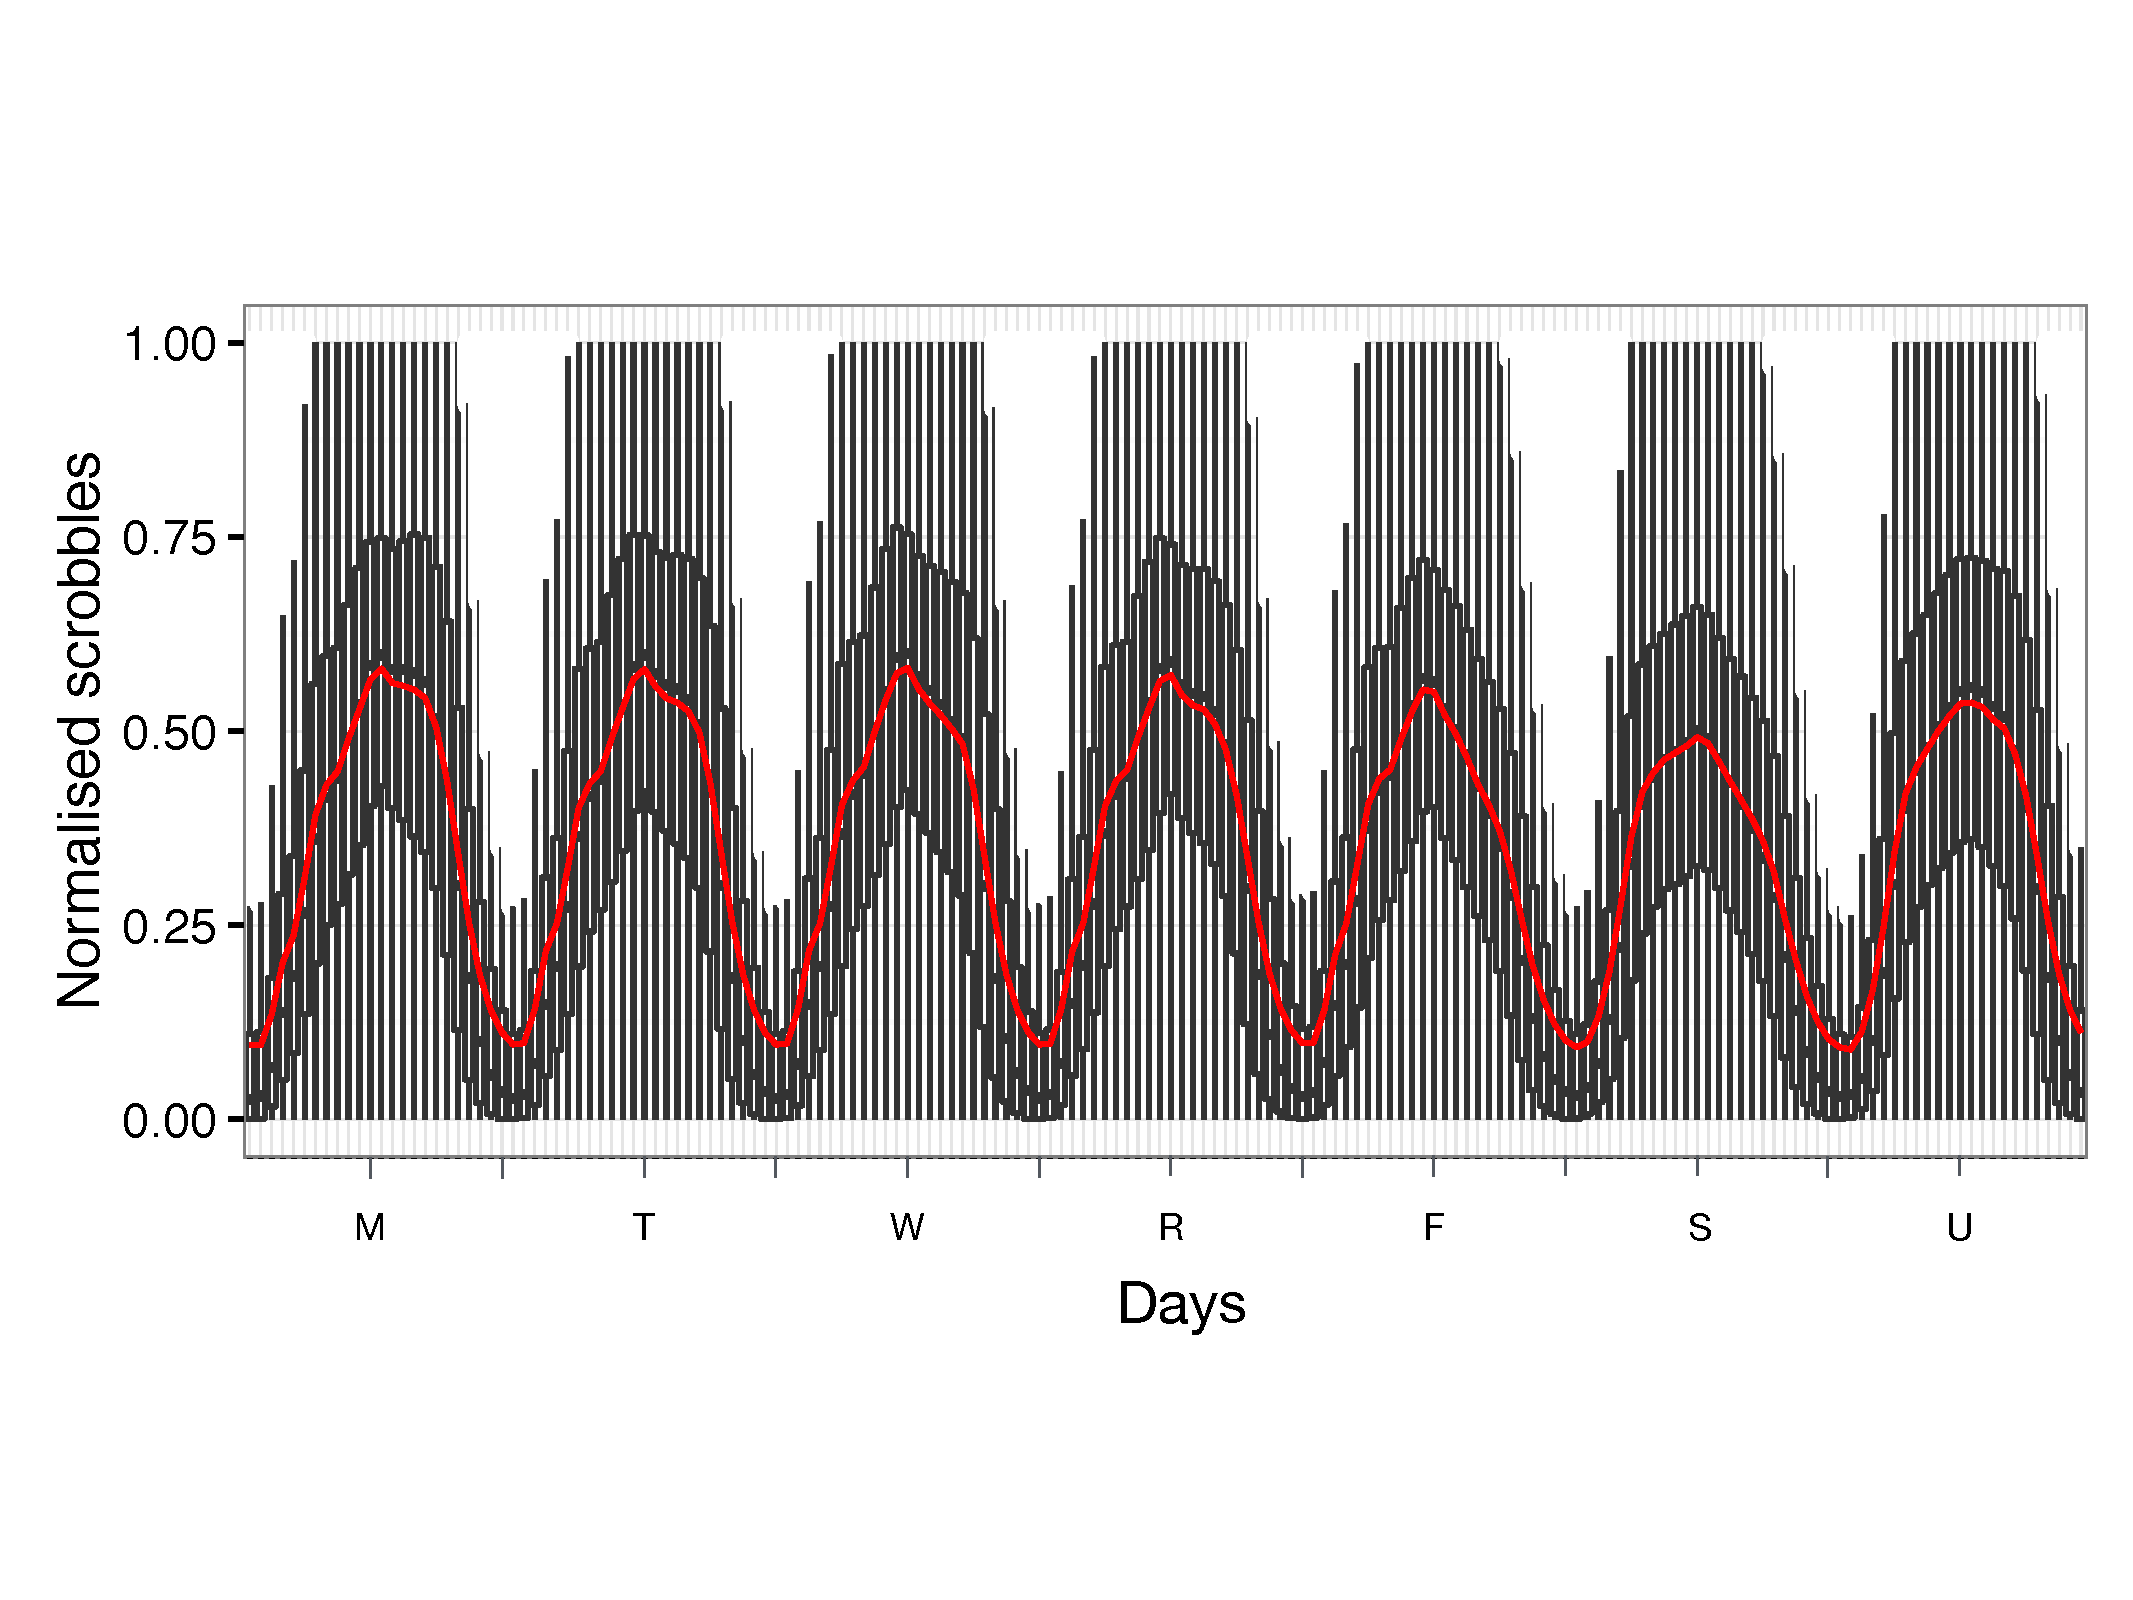
\includegraphics[width = 0.775\textwidth]{weekly_aggregated_UK_axis.jpg}
	\caption[Normalised per-week hourly aggregated number of scrobbles for UK listeners]{Normalised per-week hourly aggregated number of scrobbles for UK listeners (N = 42K). The red curve shows the normalised average number of scrobbles per hour over a week. The boxplots show median and quartiles per hour. We used this time series as the control time series for the TZ0xCORR time zone normalisation approach.}
	\label{fig:weekly_aggregated_UK_axis}
\end{figure}



These findings are contrary to what was previously reported by \textcite{north04uses}: people's exposure to music is greatest in the evening, particularly between 10 p.m. and 11 p.m., and on weekends. Furthermore, \textcite{sloboda01functions} found that people were not exposed to music at all while they were working, but mostly when they were at home. However, both studies were of a much smaller scale in terms of number of participants and the length of the period of music listening histories covered. 
Furthermore, those studies were developed more than a decade ago and music consumption behaviour has since changed to a very great extent. 
Music is nowadays consumed ubiquitously by means of portable devices accessing music streams through the Internet, and listeners seem to be willing to pay, or be exposed to ads, for accessing these services \autocite{wikstrom13music}. This behavioural change implies that people now can listen to music in any place with an Internet connection.

% there is no overlap between the CI error bars for peak and valleys in day and night, and so we found statistically significance support to our second assumption that stated that listeners generated less music logs songs during the night time than during the day.

We decided that the behavioural changes observed in the weekly aggregation preserved more information than the daily aggregation series. As a result, we decided to use the weekly time series as the control time series to estimate world users time zones using the TZ0xCORR approach.
Hence, we computed the lag in the number of hours needed to obtain the highest correlation between each user's aggregated music listening history and the TZ0 users control time series. 





% \begin{figure}[ht!]
% \vspace{1em}
% \centering
% \includegraphics[width = 0.75\textwidth]{5_clusters_20K.png}
% \caption{Clusters of listener's daily listening profile.}
% \label{fig:cluster_listeners}
% \end{figure}



% USING THE DAILY APPROACH INSTEAD OF THE WEEKLY ONE GAVE A LARGER PEAK AT TZ0, check http://thr.vigliensoni.com/?paged=6

% Also, check all the development blogged in http://thr.vigliensoni.com/?paged=6

In Figure \ref{fig:listenerstimezonebytz0weeklycorrelation} we show the estimated distribution of the overall listeners' time zones.	
\begin{figure}[!h]
% \vspace{1em}
\centering
\includegraphics[width = 0.9\textwidth]{listeners_tz_xcorr.pdf}
\caption[Distribution of the time zones for all users of the dataset]{Distribution of the time zones for all users of the dataset (N = 594K), estimated with cross correlation between their hourly weekly aggregated music listening histories and the average music listening histories from users in time zone 0.}
\label{fig:listenerstimezonebytz0weeklycorrelation}
\end{figure}
We can see a peak in the estimated time zone from where people was scrobbling at time zone GMT +0, with about 17 percent of the dataset users. Although just a few countries belong to that time zone, there are many countries in the Central European time zone that may have been merged because of their time shift in the Summer time due to the observance of the daylight saving time,  which represents roughly half of the year.
Another possibility for the large peak has to do with the actual correlation process: listening histories from people in close time zones got correlated without any lag due to individual shifts in their everyday life schedule.
The figure also shows that the TZ0xCORR approach estimated that many users were at $\pm$1 GMT and that there were many people spread between [-6, -3] GMT and [+6, +11] GMT. 

All in all, a large proportion of the listeners were estimated to be within time zones corresponding to Western Europe, but also spread out throughout the different time zones in America. The dataset did not seem to have many listeners from Asia. Finally, the shape of the people's estimated time zone seems to follow the distribution of users per country we showed on Figure \ref{fig:6_listeners_per_country}, where the majority of listeners in the dataset did self-report to be in the US and Western Europe.





% \begin{figure}[htb]
% 	\hspace{-1.5em}
% 	\epsfig{file=plots/listeners_extracted_timezone.png, width=3.5in}
% 	\caption{Time zone distribution for 594K listeners when cross correlating their aggregated weekly listening history with the average profile from listeners in time zone 0.}
% 	\label{fig:listenerstimezonebytz0weeklycorrelation}
% \end{figure}






\subsubsection{Local minima approach}
Based on the assumption that there is a smaller likelihood of people scrobbling at night compared to during the day, we developed a different method to estimate the time zone of users of the dataset. 
In this approach, we searched for the local minima indexes in the weekly aggregated listening profiles.
% , with a moving neighbourhood time period of 12 hours. %GVM:???
These minimum values provided a metric about when people actually submitted fewer music logs, probably because they were sleeping. 
Since we also expected that listeners changed their behaviour slightly on weekends---being different than on weekdays---we focused our analysis in extracting the local minima in weekdays only.

We implemented this approach by using the ``Wavelet Methods for Time Series Analysis'' (WMTSA) R package.\footnote{Wavelet Methods for Time Series Analysis (WMTSA) R package available at \url{http://CRAN.R-project.org/package=wmtsa}} Starting from a time series, the {\tt wavCWTPeaks} peak detection method of the package returns a matrix with the local maxima or minima indexes and their values. We retrieved the minima indexes from the weekly aggregated listening profiles, and normalised these indexes to the range [-12, 11] in order to have them within the range of a day. 
Then, we averaged and rounded these normalised minima indexes to an integer value. This final number was assumed to correspond to the estimated time zone for each listener. 
Averaging and rounding the multi local minima points allowed us to overcome the following problems: (i) minima that were not retrieved, because the effectively retrieved points were used for the final estimation; and (ii) false positive minima, because these values were averaged with the true positives, and so their effect was minimised. 


After implementing this approach, we realised that the local minima indexes of listening profiles with ``flat zones'' (i.e., valleys in a listening profile with no substantial change for a period of time) were usually at the beginning rather than at the middle or the end of the ``flat zones.'' 
In order to address this issue, we implemented a variant of the local minima approach that computed the local minima for the original time series of the weekdays, as well as its reversed version. The indexes obtained with this backward version were reversed again, and averaged with those retrieved by the forward version.
We expected that this method would be able to estimate the index at the middle for each one of the ``flat zones.'' 
The variant that calculated the time zone based on only the forward time series was named forward local minima (FF\_LM). The approach that calculated the time zone based on the forward and backward time series was named forward-backward local minima (FB\_LM).

\begin{figure}[!h]
% \vspace{1em}
\centering
\includegraphics[width = 0.85\textwidth]{local_minima_C.pdf}
\caption[Time-zone normalisation, local minima approach and variants]{Local minima approach and variants. Red dots indicate the daily minima indexes during weekdays, blue dots indicate the daily minima of the reversed time series, and green dots the average of the forward and backward time series minima indexes. The FF\_LM time zone estimation variant was based on the integer average of red minima indexes within a day. The FB\_LM variant was based on the integer average of green minima indexes.}
\label{fig:local_minima}
\end{figure}


In Figure \ref{fig:local_minima} we show a weekly aggregated listening profile. Red dots show the found minima during weekdays, blue dots show the minima indexes using the reversed version of the time series, and green dots show the average of the forward and backward versions. The FF\_LM time zone estimation is based on the integer average of red minima indexes within a day. FB\_LM is based on the integer average of green minima indexes.



\subsection{Seasonal decomposition}
In addition to the previous experimental factors for testing the best approach to identify time zones, we also employed time series decomposition to isolate the cyclic seasonal data from any trend and noise in the weekly aggregated music listening profiles. 
In other words, we also evaluated if removing the noise and trends of the profiles would improve the performance of any of the previously detailed approaches for time zone normalisation.
As a result, we ended up with raw and seasonal variants for each of the approaches, either based on the time-zone-0 (TZ0) cross correlation, or local minima (LM). All in all, we evaluated these two different main approaches and their variants.
% : TZ0xCORR, FF\_LM, FB\_LM, SEAS\_TZ0xCORR, SEAS\_FF\_LM, SEAS\_FB\_LM. 
In Table \ref{table:TZ-method-summary-cropped} we show a summary of the different approaches and variants, as well as an brief description of each method.

\begin{table}[!h]
% \vspace{1em}
\centering
\caption{Summary of methods for time-zone normalisation.}\label{table:TZ-method-summary-cropped}
\includegraphics[width = 1.00\textwidth]{TZ-method-summary-cropped.pdf}
\end{table}

\subsection{Experimental comparison}
We designed an experiment with the purpose of comparing the performance of all the approaches and their variants in identifying the time zones where weekly aggregated music listening patterns were generated.
To accomplish our goal, we designed an experiment in which we created a ground truth of time zones by randomly selecting a subset of listening histories from the dataset, aggregating their data into a week, and manually labelling each one of these profiles in a time zone within the range [-12, 11]. We followed \textcite{cochran77sampling} and estimated that a sample size of 384 listening histories would give us 95 percent confidence interval at $\pm$5 percent error.

To annotate the time zone for each listening profile, we visually inspected the time series and carefully paid attention to the assumptions already described: (i) listeners, in general, submit fewer music logs at night; (ii) people, in general, share a common pattern of music listening. We also assumed that people's behavioural patterns of listening change on weekends and so we only paid attention to weekday cycles. We named this subset the control dataset. 

Although we expected that labelling listeners' time zones would be straightforward, we realised that their annotation was difficult. Most people in the control dataset had cyclic patters but some had slight changes in their weekly profiles. As a result, choosing one specific time zone was not obvious. Furthermore, a few listeners did not have a clear cyclic pattern at all. 
In order to exemplify some this variability, in Figure \ref{fig:tz_eight_users} we show the weekly aggregated listening profile of six listeners supposedly to be in different time zones. While it seems easy to estimate the time zone of listeners in the upper row, the annotation is problematic for the ones in the bottom row. 

\begin{figure}[!h]
\vspace{1em}
\centering
\includegraphics[width = 0.75\textwidth]{8_aggregated_weekly_behaviour.pdf}
\caption[Example of weekly aggregated music listening profiles of six listeners]{Weekly aggregated music listening profiles of six listeners in our control dataset. While the time zones for the profiles in the upper row was easily estimated by visual inspection, the estimation for the lower row profiles was problematic.}
\label{fig:tz_eight_users}
\end{figure}

After we created the control dataset, we proceeded to compute the time zones with the six aforementioned approaches. In order to evaluate the different approaches, and given the limited ``ground truth'' data, we used a bootstrapping technique. This technique makes use of re-sampling for computing an estimator such as the confidence interval or standard error when analysing small datasets with sparse prior information or unclear distributions \autocite{henderson05bootstrap}.
As a result, we took random samples with replacement from the original population of listening profiles, creating 1,000 random populations of 384 listening profiles each. 

We wanted to calculate the performance of each method not only by measuring the percentage of perfect matches between the estimated time zones and to the ones in the control dataset, but also by how close those were to each other. In other words, an error in the estimation of $\pm$1 hour should be less important than a larger difference. Hence, we quantified the performance of each approach by computing their time difference in hours. For example, if both the computed and the manually labelled weekly listening profile had the same time zone, their time difference was zero, but if the computed profile was shifted by two hours to the left, their time difference was -2 hours.



In Figure \ref{fig:1000pop_6met_mn_sd_24timediff} we show the performance of the six approaches in identifying time zones of listening profiles. 
Bars and colours indicate the time differences in hours, ranging from [-12, 11], where a zero-hour difference is orange. 95 percent CI error bars show upper and lower limits for 1,000 bootstrap samples replicated from the original sample of 384 listening histories using bootstrap at $\alpha$ = 0.05. 


\begin{figure}[!h]
% \vspace{1em}
\centering
% \epsfig{file=plots/1000_pops_6_methods_per_24_timediff_PRINT.pdf, width=\textwidth}
\includegraphics[width=1.0\textwidth]{1000_pops_6_methods_per_24_timediff_PRINT.pdf}				
\caption[Performance of six approaches for time-zone normalisation]{Performance of six approaches in identifying time zones of listening profiles. The plot shows percentage and 95\% CI error bars for each possible time difference between the manually labelled control dataset and the computed time zones for 1,000 bootstrap samples taken from 384 listening histories.}
\label{fig:1000pop_6met_mn_sd_24timediff}
\end{figure}






It can be seen in the figure that the largest percentage of correctly computed time zones (i.e., time difference was zero) was achieved by TZ0xCORR and SEAS\_TZ0xCORR, showing significant differences with the other approaches. 
However, when analysing the performance of all methods with a tolerance of $\pm$1 hour, the FB\_LM and FF\_LM approaches---methods based on the assumption that people scrobble less frequently at night---had a much better performance. In fact, these methods appropriately computed the time zones, with a one-hour window tolerance, for 75 and 70 percent of the dataset respectively. 

There was no significant difference between models for aligning local minima. Hence, the forward-backward approach we implemented to overcome the estimation of minima of listeners with ``flat zones'' was not effective. 
%In fact, if we look in Fig. \ref{fig:1000pop_6met_mn_sd_24timediff} to all four \emph{local minima}-based methods (i.e., \emph{FF\_LM}, \emph{FB\_LM}, \emph{SEAS\_FF\_LM}, and \emph{SEAS\_FB\_LM}) we can see that they peak at a time difference of $-1$. 
%Pragmatically, if we just delay the time zones by $+1$ and use any of these four methods, we will obtain an improvement of 10 percent in the time zone recognition. 
The seasonally decomposed versions of the local minima approaches had a poorer performance than their raw counterpart, implying that there was information in the full data that was lost when we decomposed the time series. This data may be helpful for determining the time series of the weekly time series and so it should not be discarded.
Overall, the best approach was based on finding the local minima of weekly aggregated listening profiles, which was based on the assumption that people share hours of sleep at night. This approach recognised correctly 75 percent of the time zones with $\pm$1 hour of tolerance. 

Some drawbacks may be raised concerning our experimental design and analysis. 
First, the time zone of listeners can be not fixed, especially when considering long listening histories. People may travel for vacations or work while still being submitting music logs, or they may move to a different time zone indefinitely. Although the aggregation of long listening histories minimises the former issue, it can not cope with the latter. Also, this approach may also be biased against workers who work a night shift. It would be interesting to investigate the actual percentage of people migrating to different time zones and working a night shift, and see if this point could have an effect in our analysis. 


Second, in spite of the fact that individual schedule variation (e.g., morning people as opposed to night people) could possibly exceed small differences in time zones, the approaches we designed for identifying time zones in people's listening profiles can still be used to know the shift of these cyclic listening patterns in time, allowing straightforward comparison between them. 
As a consequence, having the listening histories aligned in time permits to easy comparison of listening patterns because the shift between them will be minimised. This may be helpful, for example, to profile listeners by the proportion of listening logs they submit during a day or a week. This may provide a degree of information about people's listening habits, data that could be used as a signal that may be used by music recommendation services to tailor their recommendations to the specific situation of the listener.


In this chapter we described the creation of the MLHD, a very large dataset of full music listening histories. We presented the criteria for the data collection, acquisition, cleaning, and the integration of the data. We then provided insights about the demographic characteristics of users in the dataset, and we investigated about different approaches for performing a temporal alignment of the music listening histories that will allow us to compare them directly.

In the next chapter we will formalise a set of features to describe some of the aspects of the music listening behaviour of listeners in the MLHD, and we will show different patterns of these features that can be found at the country, age, and gender level. 
We will finalise the next chapter by evaluating whether the demographic, profiling, as well as contextual features extracted from the music listening histories can improve the accuracy of a series of music artist recommendation models.

% \subsection{Temporal distribution of music logs}
% Analysing the temporal distribution of music logs shows that listeners in our dataset are less active during night, as expected, but there was no significant difference between days of the week. This distribution of music logs per hour of the day and the of the week is similar to other music listening behaviour datasets, such as the MMTD \textcite{hauger13million}.
% TODO: write about the weekly aggregated temporal distribution. 

% TODO: write about the clustering of daily and weekly aggregated music listening histories. how they cluster and why i did not use them for profiling users in the dataset. Ex: http://thr.vigliensoni.com/?paged=5



% \section{Conclusions}\label{sec:5-conclusions}
% TODO!!!!





















